\documentclass[conference]{IEEEtran}
\usepackage{config/ieee-paper}
\usepackage{lipsum}
\input{config/hyphenation}
% Adding references to the document
\addbibresource{IEEEabrv.bib}
\addbibresource{references.bib}
\IEEEoverridecommandlockouts{}
% The preceding line is only needed to identify funding in the first footnote. If that is unneeded, please comment it out.
\begin{document}
\title{CSC730: Assignment 8\\How many labels do we really need, anyway?\\Active Learning}
\author{\IEEEauthorblockN{Kristophor Ray Jensen}
    \IEEEauthorblockA{\textit{Electrical Engineering and Computer Science} \\
        \textit{South Dakota School of Mines and Technology}\\
        Rapid City, United States \\
        0009-0001-7344-349X}

}
\maketitle
\section{Introduction}
Anomaly detection is a crucial task in various domains, from fraud detection in financial transactions to identifying rare diseases in medical diagnosis. Traditional anomaly detection methods often focus on profiling normal instances and identifying instances that deviate from this normal profile. However, a novel approach called Isolation Forest (iForest) takes a fundamentally different approach by explicitly isolating anomalies instead of profiling normal points \cite{liu2008isolation}.

The requirements for this assignment are as follows\cite{assignment7}.\par
\begin{enumerate}
    \item Get the provided dataset from D2L.
    \item Write your own version of isolation forest code.
    \item Run your code on the dataset to obtain anomalousness scores for each point for your chosen parameter settings.
    \item Sort the points by anomalousness scores and generate a precision-recall curve.
    \item Generate the equivalent of the following figure from your forest.
    
\end{enumerate}

In this assignment, we implement the Isolation Forest algorithm from scratch and evaluate its performance on a dataset provided by the instructor. The dataset contains normal and anomalous instances, and our goal is to assess the effectiveness of the Isolation Forest algorithm in detecting anomalies.
\section{Methodology}

\subsection{Data Preparation}
There were two phases attempted during this assignment to aid in understanding. The first set of algorithms used worked with the following data sets: 
\begin{itemize}
    \item Raw Data
    \item PCA 2d
    \item PCA 3d
    \item PCA 4d
    \item PCA 5d
    \item t-SNE 2d
    \item t-SNE 3D
\end{itemize}

Many algorithms were run against these data sets and the results are graphed in the appendix.\par
The second phase of our discovery for this assignment used the following data sets:

\begin{itemize}
    \item Raw Data
    \item PCA 10d
    \item t-SNE 3d
    \item t-SNE 2d
\end{itemize}

We will refer the reader to the Jupyter notebook to align the results of the of the first phase to the graphs in the appendix. The training runs took many hours and were reduced to the following algorithms to increase consistency.\par


\subsection{Active Learning Rare Class Discovery}
For the active learning rare class discovery algorithm, we implemented the following query strategies:
\begin{itemize}
    \item Uncertainty Sampling
    \item Mahalanobis Uncertainty Sampling
    \item Random Sampling
\end{itemize}
These query strategies were stored in the \texttt{strategies} list.

Additionally, we used the following classifier models for the active learning algorithm:
\begin{itemize}
    \item K-Nearest Neighbors with k=10
    \item Random Forest
    \item Support Vector Machine
\end{itemize}
These models were stored in the \texttt{models} list.

\subsection{Visualization}
To gain insights into the structure of the datasets, we visualized the data using 2D and 3D t-SNE projections. The 2D t-SNE plots are shown in Figure~\ref{fig:tsne_2d}, and the 3D t-SNE plots are shown in Figure~\ref{fig:tsne_3d}. The 3D t-SNE visualization is also provided as a MP4 movie to allow for interactive exploration of the data.\par
We also generated an animation of the 3D t-SNE visualization to provide a more interactive and dynamic view of the data. This animation allows for a more detailed exploration of the data, revealing potential clusters and outliers that may not be as apparent in static visualizations.
\begin{figure}[htbp]
\centering
\includegraphics[width=0.5\textwidth]{resources/images/tsne_2d.png}
\caption{2D t-SNE Visualization of the Dataset}
\label{fig:tsne_2d}
\end{figure}

\begin{figure}[htbp]
\centering
\includegraphics[width=0.5\textwidth]{resources/images/tsne_3d.png}
\caption{3D t-SNE Visualization of the Dataset}
\label{fig:tsne_3d}
\end{figure}
One requirment of our assignment was to review the clustering accuracy of the fuzzy c-means algorithm as applied to the skewed MNIST dataset.
The fuzzy c-means algorithm is a clustering algorithm that is based on the minimization of the objective function. 
The objective function is a function that is used to measure the quality of a clustering. The objective function was defined above in equation~\ref{eq:objective_function}.
When clustering is finished we need to compare the clusters that were produced to the actual labels of the data. We will use the rand index to compare the clusters to the labels. The rand index is defined as follows:
\begin{equation}
\label{eq:rand_index}
RI = \frac{n_{00} + n_{11}}{n_{00} + n_{11} +n_{01} + n_{10}} = \frac{n_{00} + n_{11}}{{n \choose 2}}
\end{equation}
where $n_{11}$ is the number of pairs of elements that are in the same cluster and in the same class, $n_{00}$ is the number of pairs of elements that are in different clusters and in different classes, and ${n} \choose {2}$ is the total number of pairs of elements in the dataset. 
The rand index is a value between 0 and 1. 
A value of 1 indicates that the clusters are identical to the labels.
A value of 0 indicates that the clusters are completely different from the labels. 
The rand index is a good measure of the accuracy of the clustering algorithm. 

While the FCM algorithm was running, we decided to review the progression of J~\ref{eq:objective_function}.

\begin{figure}[H]
    \centering
    \includegraphics[width=0.5\textwidth]{objective_function_iterations.png}
    \caption{St. Dev. Normalized obejective functions through runtime of the FCM algorithm}
    \label{fig:objective_function_iterations}    
\end{figure}

The RI results for the full data set resulted in a value of 0.692 and the PCA dataset resulted in a value of 0.672.

We also plotted the results of FCM applied to the PCA dataset. The clusters are graphed according by color according to their class label. 
There is also a black X to indicate the cluster center.

\begin{figure}[H]
    \centering
    \includegraphics[width=0.5\textwidth]{pca_cluster_means.png}
    \caption{Clusters produced by FCM applied to the PCA dataset}
    \label{fig:pca_clusters}
\end{figure}







The algorithm achieved mixed results. The clusters used for this example were spread out to ensure the workings of the algorithm were correct, but in a real world application, this would not always be the case.
The demo code used for the Optigrid implementation could be further improved if it allowed for cutting planes that are not all orthonormal to one another. In this way, more amorphous clusters could be split up across complex dimensions.

This project improved our knowledge of the Optigrid algorithm and of each of the algorithm's parts. Through documenting the example code given via deep description, we extended our understanding of the algorithm past that of just writing code about it.
By experimenting with the demo code, we also expanded our use case of external repositories and libraries in order to produce a new result. 
Overall, this project helped us learn more about the Optigrid algorithm and how to use it for unsupervised learning.
\printbibliography{}

\newpage
\onecolumn
%\appendix

%return to single column

\section{Appendix: Isolation Forest Tree Visualizations}

\begin{figure}[htbp]
\centering
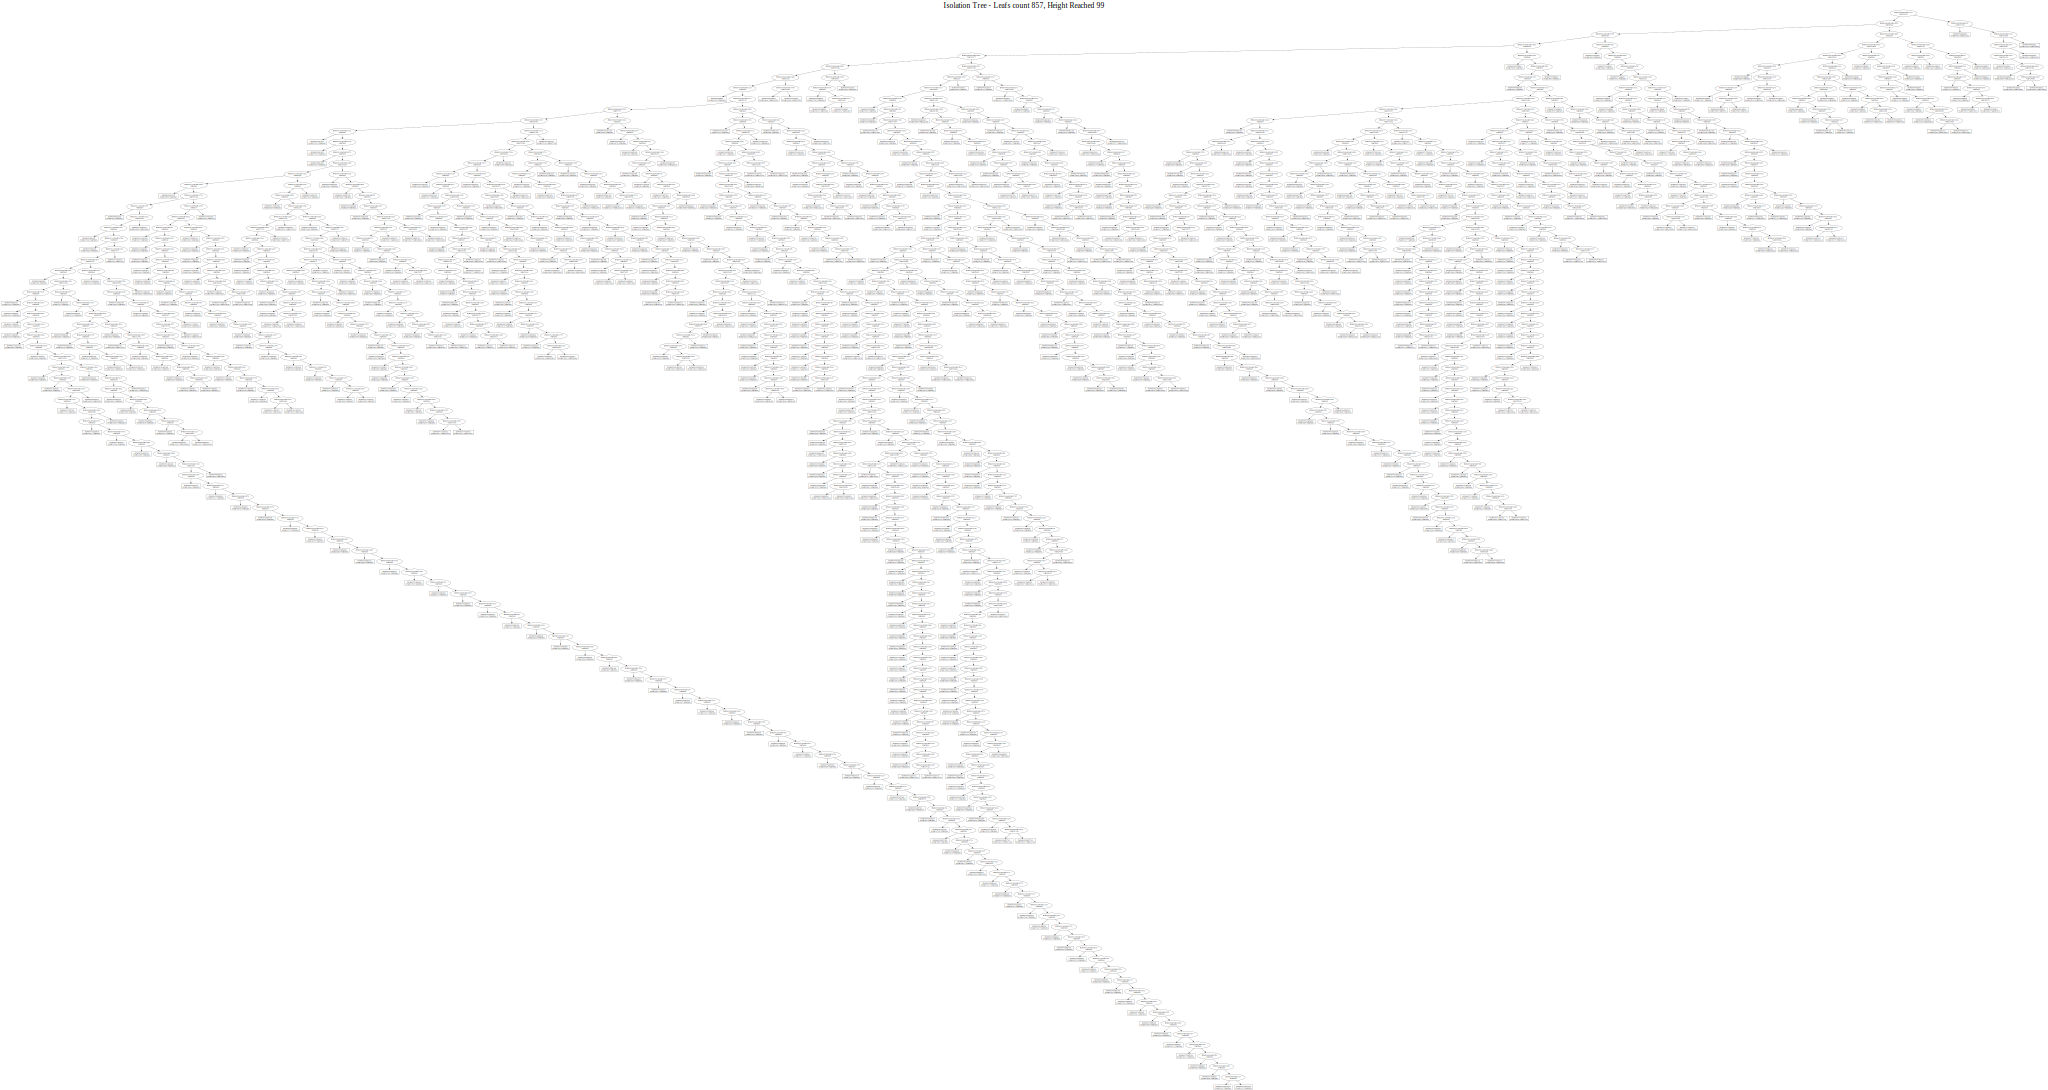
\includegraphics[width=1\textwidth]{resources/images/itree_graph.png}
\caption{Visualization of an Isolation Tree (iTree)}
\label{fig:itree_appendix}
\end{figure}

\begin{figure}[htbp]
\centering
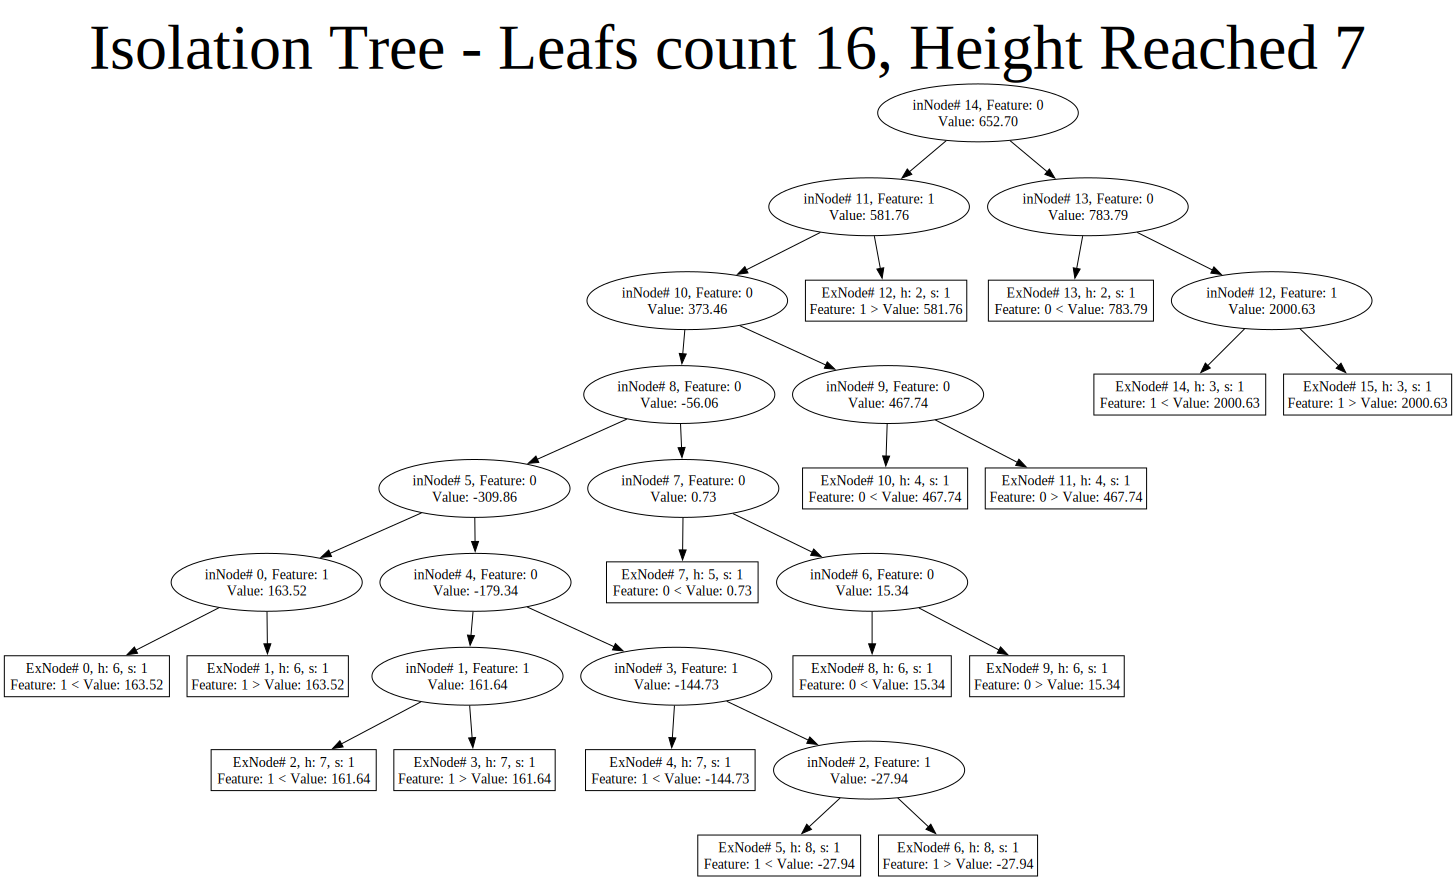
\includegraphics[width=1\textwidth]{resources/images/itree_pca_graph.png}
\caption{Visualization of an iTree with PCA}
\label{fig:pca_itree_appendix}
\end{figure}

\begin{figure}[htbp]
\centering
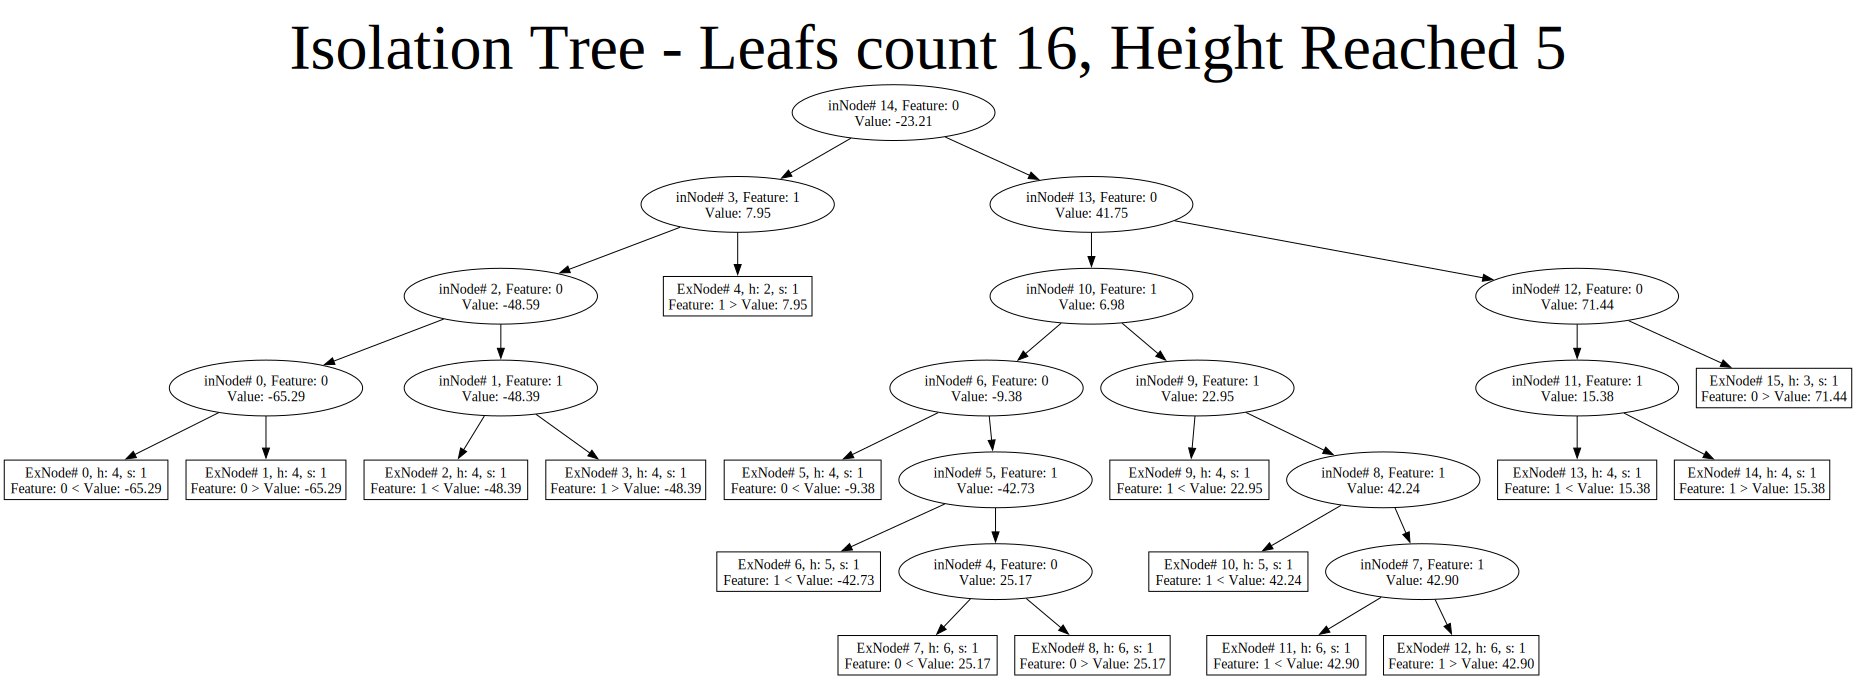
\includegraphics[width=1\textwidth]{resources/images/itree_tsne_graph.png}
\caption{Visualization of an iTree with t-SNE}
\label{fig:tsne_itree_appendix}
\end{figure}
\vspace{12pt}
\end{document}
